\begin{frame}[t]{\secname}%{\subsecname}
  
\begin{columns}[t]
  \begin{column}{0.57\textwidth}
    \begin{itemize}
      \item<1-> Challenges:
        \begin{itemize}
          \item<1-> Exploitation of fiber reinforced plastics (FRP) lightweight potential limited
          \item<1-> Missing reliability of failure predictions
        \end{itemize}
      \item<2-> Goals:
        \begin{itemize}
          \item<2-> Increase understanding of failure mechanisms
          \item<2-> Derive improved failure criteria for preliminary design
        \end{itemize}
      \item<3-> Use case: 
        \begin{itemize}
          \item<3-> Matrix failure in FRP
          \item<3-> Origin of other failure phenomena
        \end{itemize}
    \end{itemize}
  \end{column}
  \begin{column}{0.43\textwidth}
    \only<1|handout:0>{
      \begin{figure}
        \centering
        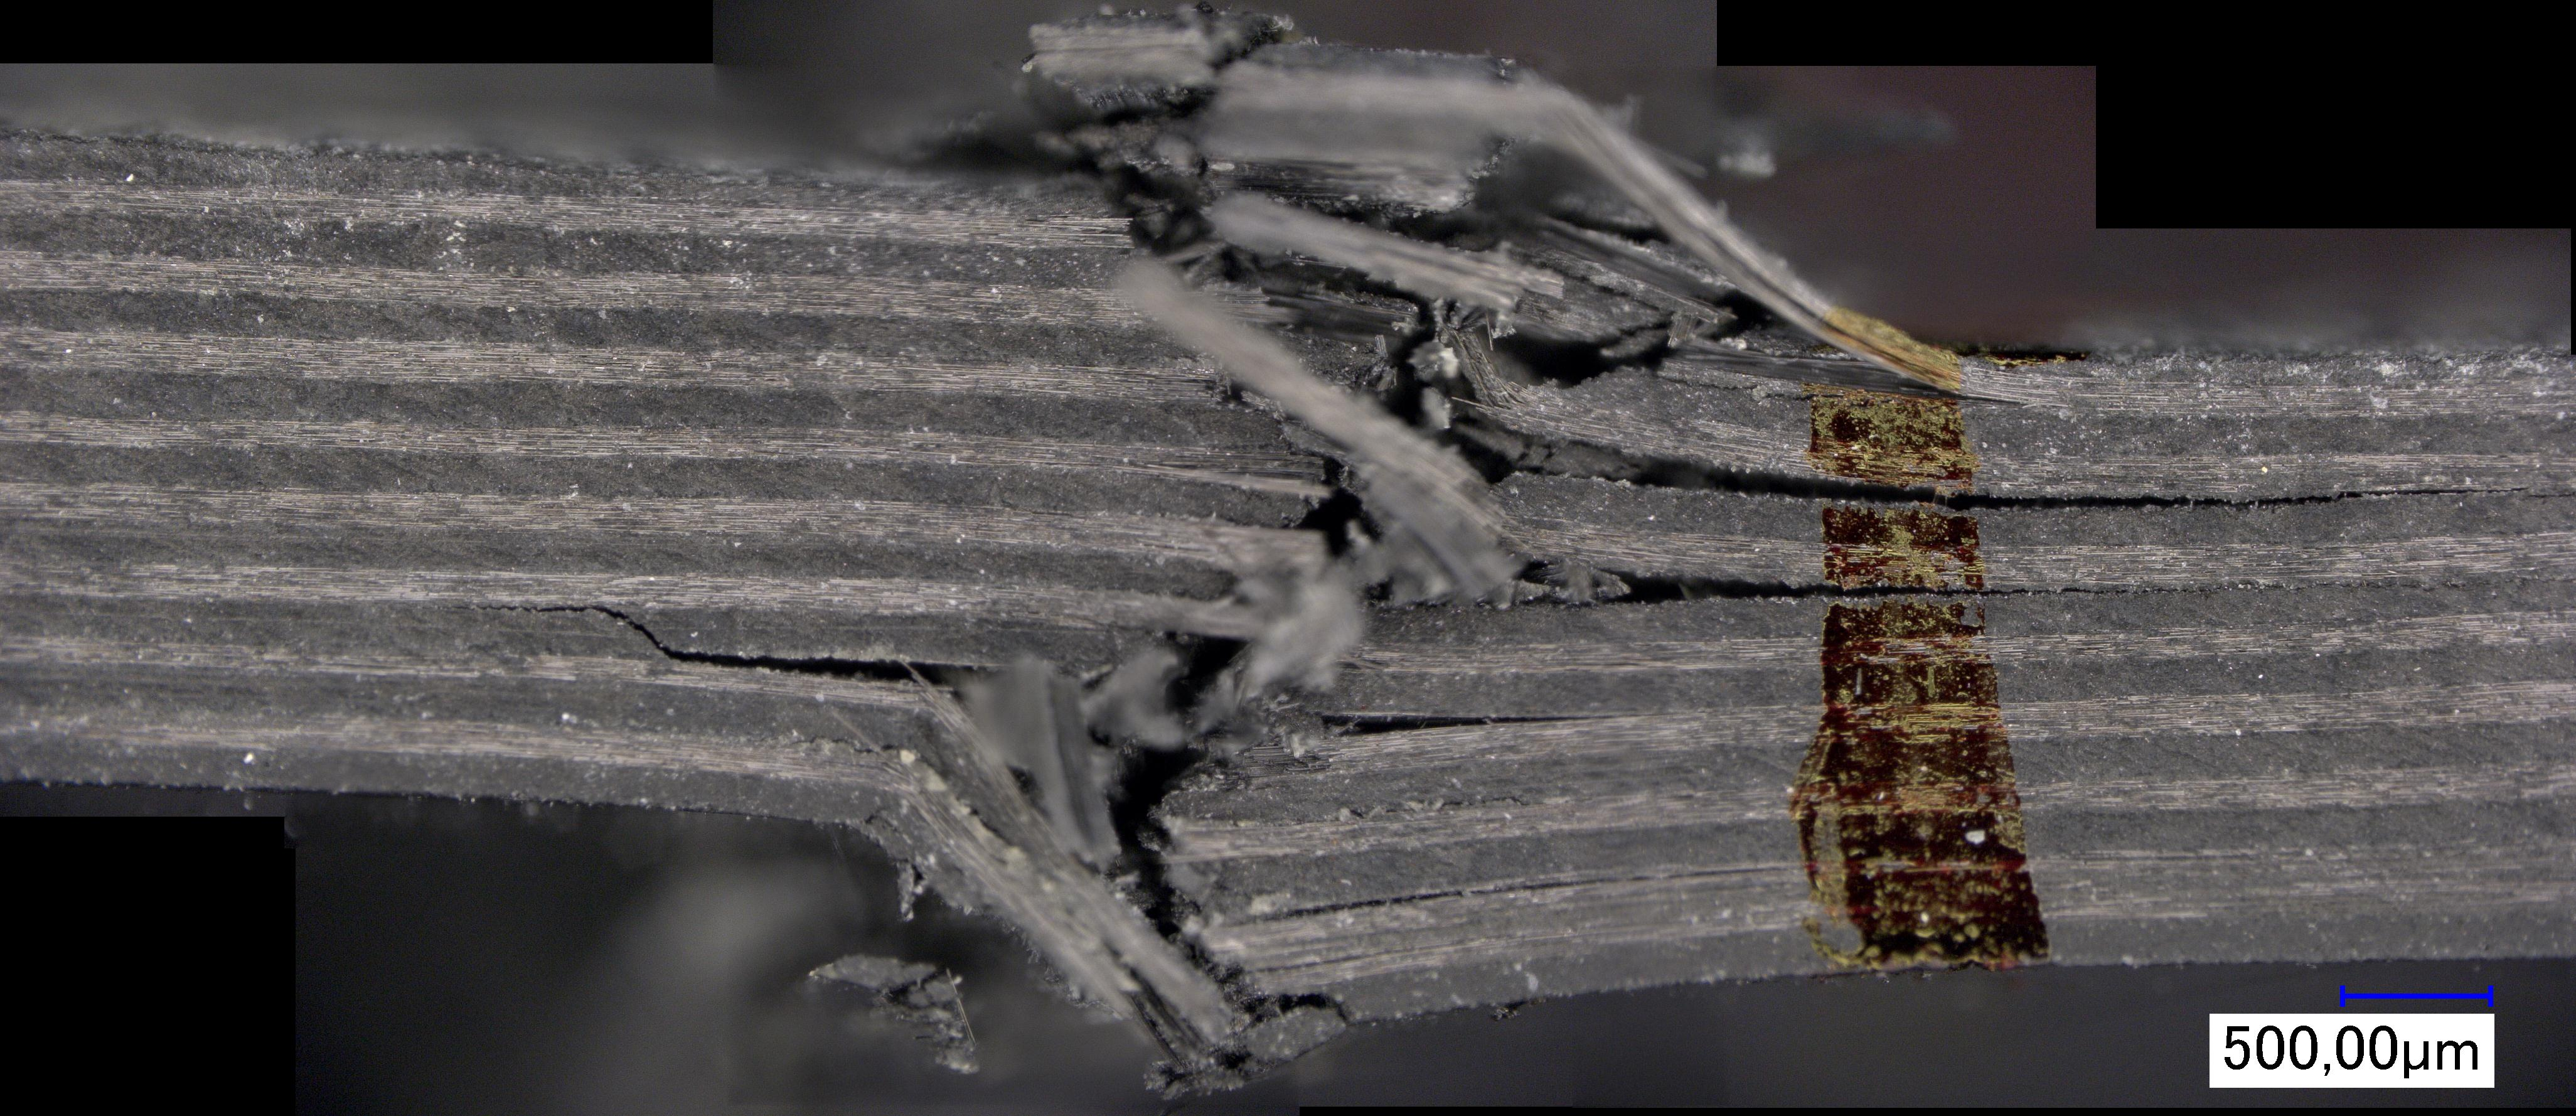
\includegraphics[width=\linewidth,keepaspectratio]{AFP-C-Gu-4-nB-v_by_Falk.jpg}
        \caption{Crack in CFRP specimen}
      \end{figure}
    }
    \only<2|handout:1>{
      \begin{figure}
        \centering
        \begin{tikzpicture}
          % External graphics
          \node[anchor=south west,inner sep=0] (image) at (0,0) {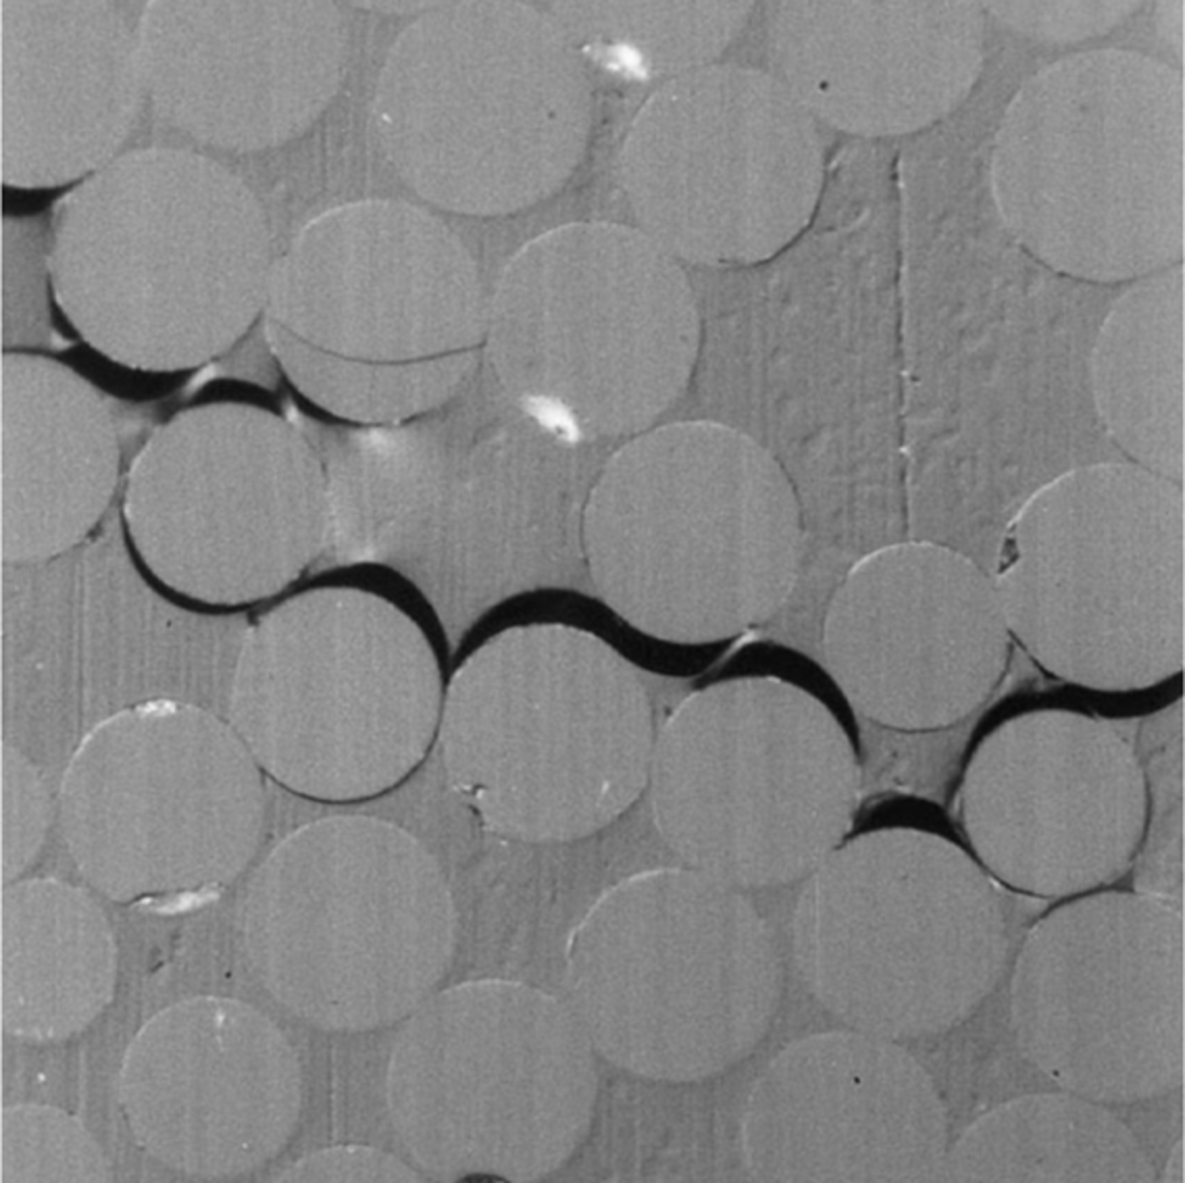
\includegraphics[width=0.75\linewidth,keepaspectratio]{Exp_Matrix_Failure}};
          % Scope
          \begin{scope}[
            x={(image.south east)},
            y={(image.north west)},
          ]
            % Arrows
            \draw[-latex,very thick] ($(image.north)+(0,0.2ex)$) -- ($(image.north)+(0,2.5ex)$);
            \draw[-latex,very thick] ($(image.south)-(0,0.2ex)$) -- ($(image.south)-(0,2.5ex)$);
          \end{scope}
        \end{tikzpicture}
        \caption{Matrix failure in FRP \cite{KrauseD2016}}
      \end{figure}
    }
    \only<3|handout:0>{
      \begin{figure}
        \centering
        \begin{tikzpicture}
          % External graphics
          \node[anchor=south west,inner sep=0] (image) at (0,0) {
\includegraphics[width=0.75\linewidth,keepaspectratio]{Model_FE_RVE_Fatigue_ct.png}};
          % Scope
          \begin{scope}[
            x={(image.south east)},
            y={(image.north west)},
          ]
            % Labels
            \node[font=\figurefontsize] (fibrelabel)     at (0.15,1.075) {Fibre};
            \node[font=\figurefontsize] (interfacelabel) at (0.50,1.075) {Interface};
            \node[font=\figurefontsize] (resinlabel)     at (0.85,1.075) {Resin};
            % Arrows
            \draw[-latex] (fibrelabel)     -- (0.125,0.825);
            \draw[-latex] (interfacelabel) -- (0.520,0.820);
            \draw[-latex] (resinlabel)     -- (0.800,0.950);
          \end{scope}
        \end{tikzpicture}
        \caption{RVE model generator \cite{KrauseD2016}}
      \end{figure}
    }
  \end{column}
\end{columns}

\end{frame}
